\documentclass{templateNote}
\usepackage{tcolorbox}
\usepackage{hyperref}
\usepackage{amsmath}
\usepackage{amssymb}
\usepackage{soul}
\usepackage{circuitikz}
% \usepackage{parskip} % Para evitar la indentation y mejorar la separación entre párrafos


\begin{document}
\imagenlogoU{img/logoUBBsintext.png}
\imagenlogoD{img/cimubbwhite.png}
\linklogoU{https://www.ubiobio.cl/w/} 
\linklogoD{https://www.ubiobio.cl/w/}
% \imagenlogoD{img/logo-ubb-txt-face.png} 
\titulo{Recopilación datos sonómetro}
\asignatura{}
% \autor{
%     \indent
%     Nicolás {Gómez Morgado}
% }


\portada
\margenes
\newpage 
\tableofcontents

\newpage
\section{Introducción}
Este informe tiene como objetivo presentar los resultados obtenidos a partir de la recopilación de datos realizada con sonómetros ubicados en cursos de enseñanza básica en la ciudad de Chillán. Los datos presentados ejemplifican la eficacia y utilidad de los sonómetros para medir el nivel de ruido ambiental y otros factores. Los datos fueron procesados y separados para poder generar gráficas independientes de tal manera que el investigador pueda comparar entre ellas y sus datos capturados para una mejor comprensión del investigador mismo.
\newpage
\section{Datos obtenidos}
Los datos recopilados durante un día de trabajo en la escuela básica son extensos, ya que el dispositivo se configuró para capturar información en intervalos de 5 segundos para todos los datos. Por esta razón, solo se adjuntará una parte de los datos. Si necesita acceder a la totalidad de la información, puede consultarla en el siguiente enlace: 
\begin{center}
    \url{https://docs.google.com/spreadsheets/d/1TQj_2DI2-8oq5jQI647WowAo7y3ISKQ6/edit?usp=sharing&ouid=108699568632162366719&rtpof=true&sd=true}
\end{center}

\noindent Es importante tener en cuenta que los datos presentados corresponden únicamente al dia 14 de agosto de 2024. Contar con un mayor volumen de datos recopilados en un período más amplio permitirá obtener conclusiones más precisas.
\\Para el dispositivo numero 1, en el periodo con mas cantidad de ocupantes, se obtuvieron los siguientes datos:

\begin{table}[H]
    \centering
        \begin{tabular}{|c|c|c|c|c|}
        \hline
            Hora    & Temperatura & Humedad & CO2 & Ruido \\ \hline
            08:10:01 & 17,39 & 61,58 & 863,69 & 81 \\ \hline
            08:10:06 & 17,38 & 61,66 & 869,34 & 81 \\ \hline
            08:10:11 & 17,41 & 61,71 & 871,18 & 82 \\ \hline
            08:10:16 & 17,41 & 61,73 & 877,76 & 80 \\ \hline
            08:10:21 & 17,42 & 61,80 & 883,06 & 82 \\ \hline
            08:10:26 & 17,43 & 62,48 & 897,41 & 80 \\ \hline
            08:10:32 & 17,45 & 64,65 & 973,94 & 83 \\ \hline
            08:10:37 & 17,45 & 64,16 & 1107,15 & 80 \\ \hline
            08:10:42 & 17,48 & 64,02 & 1363,33 & 83 \\ \hline
            08:10:47 & 17,53 & 65,01 & 1488,03 & 83 \\ \hline
            08:10:52 & 17,50 & 65,05 & 1486,89 & 80 \\ \hline
            08:10:57 & 17,53 & 64,39 & 1464,09 & 80 \\ \hline
            08:11:02 & 17,53 & 63,97 & 1432,53 & 80 \\ \hline
            08:11:07 & 17,58 & 63,46 & 1353,82 & 80 \\ \hline
            08:11:12 & 17,53 & 63,17 & 1252,11 & 80 \\ \hline
            08:11:17 & 17,56 & 62,82 & 1175,46 & 80 \\ \hline
            08:11:22 & 17,58 & 62,48 & 1160,19 & 80 \\ \hline
            08:11:27 & 17,59 & 62,35 & 1133,32 & 82 \\ \hline
            08:11:32 & 17,59 & 62,28 & 1119,77 & 80 \\ \hline
            08:11:37 & 17,59 & 62,22 & 1111,13 & 81 \\ \hline
            08:11:42 & 17,59 & 62,43 & 1113,05 & 80 \\ \hline
            08:11:47 & 17,61 & 62,38 & 1113,32 & 81 \\ \hline
            08:11:52 & 17,62 & 62,10 & 1116,03 & 81 \\ \hline
            08:11:57 & 17,62 & 61,67 & 1113,92 & 80 \\ \hline
            08:12:03 & 17,64 & 61,57 & 1107,68 & 81 \\ \hline
        \end{tabular}
    \caption{Datos capturados entre las 08:10:01 y 08:12:03}
    \label{tab:datos}
\end{table}

\newpage

\noindent Para el dispositivo numero 2, en el periodo con mas cantidad de ocupantes, se obtuvieron los siguientes datos:
    \begin{table}[H]
        \centering
        \begin{tabular}{|c|c|c|c|c|}
            \hline
            Hora     & Temperatura & Humedad & CO2 & Ruido \\ \hline
            12:19:30 & 20,12     & 60,50     & 1118,31   & 51        \\ \hline
            12:19:35 & 20,08     & 64,44     & 2342,17   & 51        \\ \hline
            12:19:40 & 20,11     & 62,30     & 2102,67   & 51        \\ \hline
            12:19:46 & 20,39     & 66,72     & 5240,33   & 51        \\ \hline
            12:19:51 & 20,23     & 71,77     & 5110,50   & 51        \\ \hline
            12:19:56 & 20,25     & 71,09     & 6052,37   & 51        \\ \hline
            12:20:01 & 20,25     & 69,28     & 5639,18   & 51        \\ \hline
            12:20:06 & 20,25     & 68,25     & 4467,17   & 51        \\ \hline
            12:20:11 & 20,19     & 66,26     & 3561,80   & 51        \\ \hline
            12:20:16 & 20,20     & 62,91     & 2569,32   & 51        \\ \hline
            12:20:21 & 20,20     & 61,73     & 2126,54   & 51        \\ \hline
            12:20:26 & 20,23     & 60,90     & 1792,73   & 51        \\ \hline
            12:20:31 & 20,23     & 61,58     & 1518,85   & 51        \\ \hline
            12:20:36 & 20,22     & 61,45     & 1321,45   & 51        \\ \hline
            12:20:41 & 20,20     & 61,07     & 1265,56   & 51        \\ \hline
            12:20:46 & 20,19     & 60,39     & 1237,25   & 51        \\ \hline
            12:20:51 & 20,20     & 60,24     & 1222,76   & 51        \\ \hline
            12:20:56 & 20,20     & 60,25     & 1199,38   & 51        \\ \hline
            12:21:01 & 20,22     & 60,74     & 1149,53   & 51        \\ \hline
            12:21:06 & 20,22     & 60,85     & 1077,09   & 51        \\ \hline
            12:21:11 & 20,23     & 60,77     & 1065,58   & 51        \\ \hline
            12:21:16 & 20,22     & 60,69     & 1051,51   & 51        \\ \hline
            12:21:21 & 20,22     & 60,91     & 1035,97   & 51        \\ \hline
            12:21:26 & 20,23     & 60,68     & 1031,27   & 51        \\ \hline
            12:21:32 & 20,20     & 60,21     & 1011,15   & 51        \\ \hline
            12:21:37 & 20,20     & 60,02     & 982,24    & 51        \\ \hline
            12:21:42 & 20,23     & 60,02     & 972,68    & 51        \\ \hline
            12:21:47 & 20,16     & 60,00     & 965,20    & 51        \\ \hline
            12:21:52 & 20,17     & 60,12     & 958,32    & 51        \\ \hline
            12:21:57 & 20,19     & 60,13     & 950,50    & 51        \\ \hline
            12:22:02 & 20,19     & 60,27     & 945,08    & 51        \\ \hline
            12:22:07 & 20,19     & 60,27     & 944,74    & 51        \\ \hline
            12:22:12 & 20,20     & 60,30     & 942,91    & 51        \\ \hline
            12:22:17 & 20,22     & 60,40     & 942,31    & 51        \\ \hline
            12:22:22 & 20,22     & 60,39     & 945,60    & 51        \\ \hline
        \end{tabular}
        \caption{Datos capturados entre las 12:19:30 y 12:22:22}
        \label{tab:data2}
\end{table}

\newpage
\noindent Para el dispositivo numero 3, en el periodo con mas cantidad de ocupantes, se obtuvieron los siguientes datos:
\begin{table}[H]
    \centering
    \begin{tabular}{|c|c|c|c|c|}
        \hline
        Hora     & Temperatura & Humedad & CO2 & Ruido \\ \hline
        09:29:52 & 21,21     & 64,80     & 3021,54   & 83        \\ \hline
        09:29:57 & 21,26     & 64,30     & 2958,70   & 83        \\ \hline
        09:30:02 & 21,33     & 63,99     & 2882,25   & 82        \\ \hline
        09:30:07 & 21,31     & 63,89     & 2832,63   & 83        \\ \hline
        09:30:12 & 21,34     & 63,64     & 2620,30   & 82        \\ \hline
        09:30:17 & 21,34     & 63,62     & 2665,63   & 83        \\ \hline
        09:30:22 & 21,37     & 63,52     & 2679,03   & 84        \\ \hline
        09:30:27 & 21,37     & 63,42     & 2706,17   & 82        \\ \hline
        09:30:32 & 21,40     & 63,35     & 2700,24   & 83        \\ \hline
        09:30:37 & 21,38     & 63,31     & 2703,82   & 84        \\ \hline
        09:30:42 & 21,41     & 63,31     & 2705,89   & 85        \\ \hline
        09:30:47 & 21,41     & 63,33     & 2714,42   & 82        \\ \hline
        09:30:52 & 21,41     & 63,30     & 2723,16   & 82        \\ \hline
        09:30:57 & 21,44     & 63,26     & 2728,05   & 82        \\ \hline
        09:31:03 & 21,43     & 63,16     & 2726,21   & 82        \\ \hline
        09:31:08 & 21,44     & 63,03     & 2725,37   & 84        \\ \hline
        09:31:13 & 21,43     & 62,79     & 2723,72   & 83        \\ \hline
        09:31:18 & 21,45     & 62,63     & 2719,72   & 82        \\ \hline
        09:31:23 & 21,45     & 62,58     & 2712,72   & 85        \\ \hline
        09:31:28 & 21,44     & 62,57     & 2704,87   & 82        \\ \hline
        09:31:33 & 21,44     & 62,66     & 2686,72   & 82        \\ \hline
        09:31:38 & 21,45     & 62,66     & 2688,89   & 82        \\ \hline
        09:31:43 & 21,47     & 62,63     & 2690,89   & 83        \\ \hline
        09:31:48 & 21,45     & 62,60     & 2687,51   & 82        \\ \hline
        09:31:53 & 21,45     & 62,56     & 2688,62   & 83        \\ \hline
        09:31:58 & 21,44     & 62,50     & 2686,23   & 82        \\ \hline
        09:32:03 & 21,44     & 62,48     & 2684,96   & 83        \\ \hline
        09:32:08 & 21,45     & 62,48     & 2680,77   & 84        \\ \hline
        09:32:13 & 21,45     & 62,51     & 2684,65   & 84        \\ \hline
        09:32:18 & 21,47     & 62,34     & 2680,36   & 84        \\ \hline
        09:32:23 & 21,48     & 62,20     & 2675,69   & 83        \\ \hline
        09:32:28 & 21,48     & 62,06     & 2672,57   & 82        \\ \hline
        09:32:33 & 21,45     & 61,95     & 2671,02   & 83        \\ \hline
        09:32:38 & 21,47     & 61,87     & 2669,48   & 82        \\ \hline
        09:32:43 & 21,47     & 61,96     & 2668,82   & 82        \\ \hline
        09:32:48 & 21,47     & 62,02     & 2669,01   & 82        \\ \hline
        09:32:54 & 21,45     & 62,04     & 2670,02   & 81        \\ \hline
        09:32:59 & 21,48     & 62,12     & 2670,71   & 82        \\ \hline
        09:33:04 & 21,47     & 62,07     & 2673,06   & 82        \\ \hline
        09:33:09 & 21,50     & 62,08     & 2673,32   & 82        \\ \hline
    \end{tabular}
    \caption{Datos capturados entre las 09:29:52 y 09:33:09}
    \label{tab:data3}
\end{table}    

\newpage
\noindent Y finalmente para el dispositivo numero 4, en el periodo con mas cantidad de ocupantes, se obtuvieron los siguientes datos:

\begin{table}[H]
    \centering
    \begin{tabular}{|c|c|c|c|c|}
        \hline
        Hora & Temperatura & Humedad & CO2 & Ruido \\
        \hline
        11:10:41 & 22,39 & 61,37 & 1993,49 & 82 \\\hline
        11:10:46 & 22,42 & 61,31 & 2007,71 & 82 \\\hline
        11:10:51 & 22,42 & 61,30 & 2011,30 & 82 \\\hline
        11:10:56 & 22,39 & 61,28 & 2008,43 & 82 \\\hline
        11:11:02 & 22,42 & 61,28 & 2010,49 & 82 \\\hline
        11:11:07 & 22,43 & 61,32 & 2008,58 & 82 \\\hline
        11:11:12 & 22,44 & 61,39 & 2011,00 & 84 \\\hline
        11:11:17 & 22,44 & 61,38 & 2013,85 & 82 \\\hline
        11:11:22 & 22,44 & 61,46 & 2020,33 & 82 \\\hline
        11:11:27 & 22,43 & 61,38 & 2023,49 & 83 \\\hline
        11:11:32 & 22,43 & 61,31 & 2024,49 & 82 \\\hline
        11:11:37 & 22,46 & 61,27 & 2022,17 & 82 \\\hline
        11:11:42 & 22,44 & 61,18 & 2025,42 & 82 \\\hline
        11:11:47 & 22,44 & 61,24 & 2027,34 & 82 \\\hline
        11:11:52 & 22,44 & 61,31 & 2030,29 & 82 \\\hline
        11:11:57 & 22,44 & 61,27 & 2031,70 & 82 \\\hline
        11:12:02 & 22,43 & 61,25 & 2032,13 & 82 \\\hline
        11:12:07 & 22,46 & 61,24 & 2034,77 & 84 \\\hline
        11:12:12 & 22,43 & 61,11 & 2036,45 & 82 \\\hline
        11:12:17 & 22,46 & 61,06 & 2036,40 & 82 \\\hline
        11:12:22 & 22,46 & 61,11 & 2038,75 & 83 \\\hline
        11:12:27 & 22,47 & 61,19 & 2044,38 & 82 \\\hline
        11:12:32 & 22,49 & 61,19 & 2053,25 & 82 \\\hline
        11:12:37 & 22,49 & 61,27 & 2058,34 & 82 \\\hline
        11:12:42 & 22,47 & 61,25 & 2060,40 & 82 \\\hline
        11:12:47 & 22,47 & 61,24 & 2066,20 & 82 \\\hline
        11:12:53 & 22,49 & 61,29 & 2066,78 & 82 \\\hline
        11:12:58 & 22,47 & 61,28 & 2074,00 & 83 \\\hline
        11:13:03 & 22,46 & 61,34 & 2072,30 & 82 \\\hline
        11:13:08 & 22,49 & 61,55 & 2076,25 & 82 \\\hline
        11:13:13 & 22,52 & 61,67 & 2079,71 & 82 \\\hline
        11:13:18 & 22,50 & 61,56 & 2081,24 & 82 \\\hline
    \end{tabular}
    \caption{Datos capturados entre las 11:10:40 y 11:13:18}
    \label{tab:data4}
\end{table}

\noindent Considerar dos aspectos importantes: en primer lugar, los datos presentados corresponden a períodos de mayor cantidad de ocupantes, ya que durante estos momentos se registran los niveles más altos de CO2. En segundo lugar, aunque se construyeron cinco dispositivos, solo se presentan los datos de cuatro de ellos, ya que el quinto dispositivo no fue utilizado en esta recopilación de datos.

\newpage
\section{Gráficas obtenidas}
Para facilitar el análisis de los datos, se construyeron gráficas que permiten una mejor visualización de la información obtenida. En el caso de las gráficas de ruido, se consideraron todos los datos del período de muestra, lo que puede resultar en una visualización más saturada en comparación con otras gráficas. Por otro lado, para las gráficas de temperatura, humedad y concentración de CO2, solo se incluyeron dato0s en intervalos de 15 minutos, ya que estos parámetros no presentan variaciones significativas en períodos cortos de tiempo.

Es importante tener en cuenta que ninguno de los dispositivos probados registró datos durante toda la sesión del tercer periodo.

\subsection{Dispositivo 1}

\textbf{Ruido}
\begin{figure}[H]
    \centering
    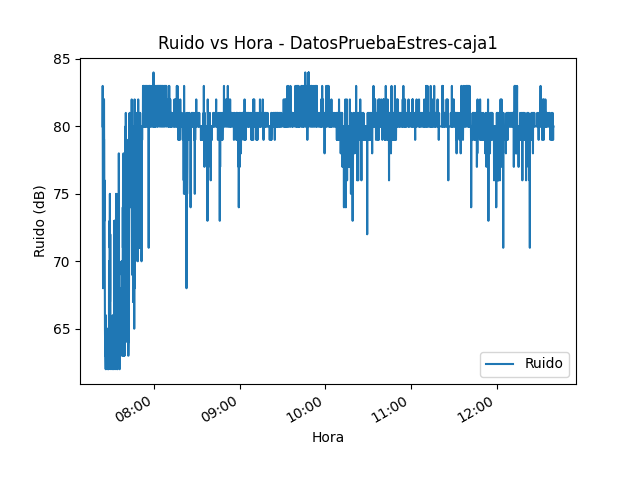
\includegraphics[width=0.8\textwidth]{img/DatosPruebaEstres-caja1_ruido_vs_hora.png}
\end{figure}

\begin{tcolorbox}
    En el caso del dispositivo 1, la gráfica de ruido muestra un inicio con valores que oscilan entre 60 y 70 dB, con algunos picos que alcanzan los 80 dB. A medida que avanza la mañana, el nivel de ruido se estabiliza en un rango constante de 80 dB, con pocas variaciones.
\end{tcolorbox}

% \begin{figure}[htbp]
%     \begin{minipage}{0.5\textwidth}
%         \centering
%         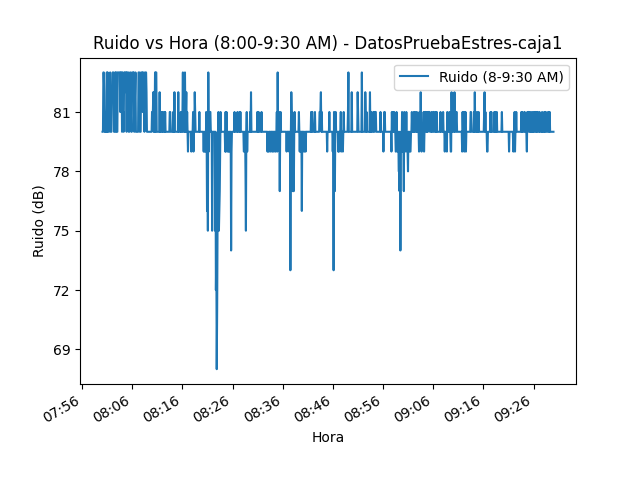
\includegraphics[width=\linewidth]{img/DatosPruebaEstres-caja1_ruido_8_9-30_am.png}
%         \caption{Primer Periodo de clases}
%         \label{fig:imagen1}
%     \end{minipage}\hfill
%     \begin{minipage}{0.5\textwidth}
%         \centering
%         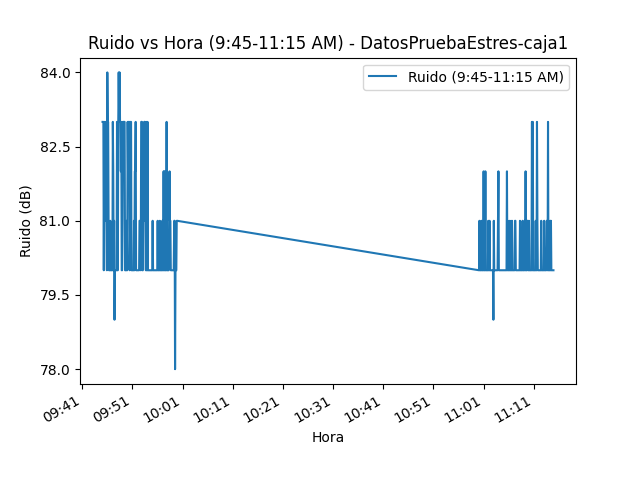
\includegraphics[width=\linewidth]{img/DatosPruebaEstres-caja1_ruido_9-45_11-15_am.png}
%         \caption{Segundo Periodo de clases}
%         \label{fig:imagen2}
%     \end{minipage}\hfill
% \end{figure}

% \begin{figure}[H]
%     \centering
%     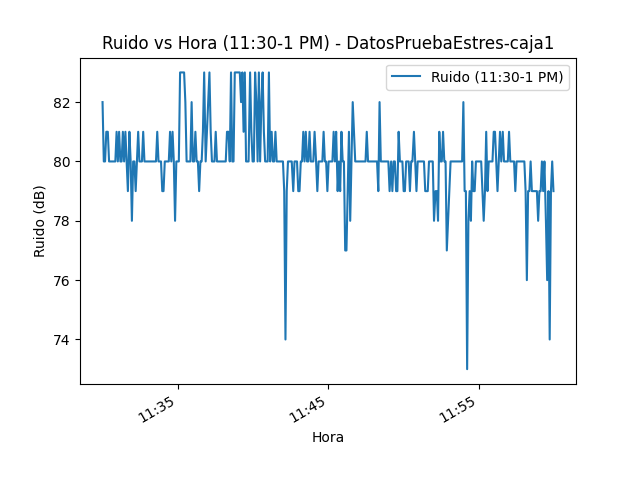
\includegraphics[width=0.55\textwidth]{img/DatosPruebaEstres-caja1_ruido_11-30_1_pm.png}
%     \caption{Tercer Periodo de clases}
%     \label{fig:imagen3}
% \end{figure}

\newpage
\underline{Graficas por periodos de clases:}

\begin{figure}[H]
    \centering
    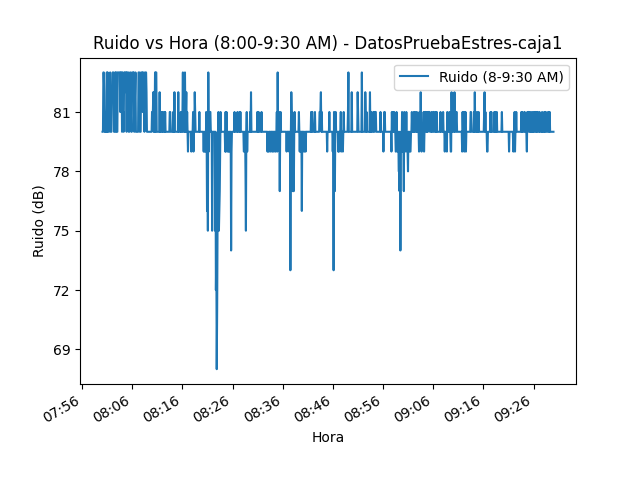
\includegraphics[width=0.8\textwidth]{img/DatosPruebaEstres-caja1_ruido_8_9-30_am.png}
    \caption{Primer Periodo de clases}
\end{figure}

\begin{figure}[H]
    \centering
    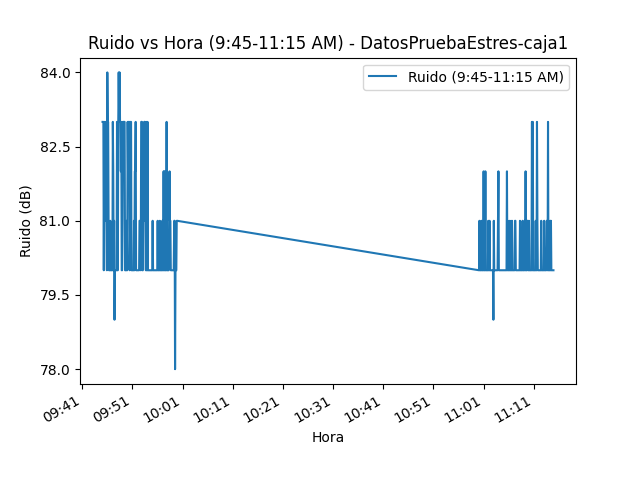
\includegraphics[width=0.8\textwidth]{img/DatosPruebaEstres-caja1_ruido_9-45_11-15_am.png}
    \caption{Segundo Periodo de clases}
\end{figure}

\begin{figure}[H]
    \centering
    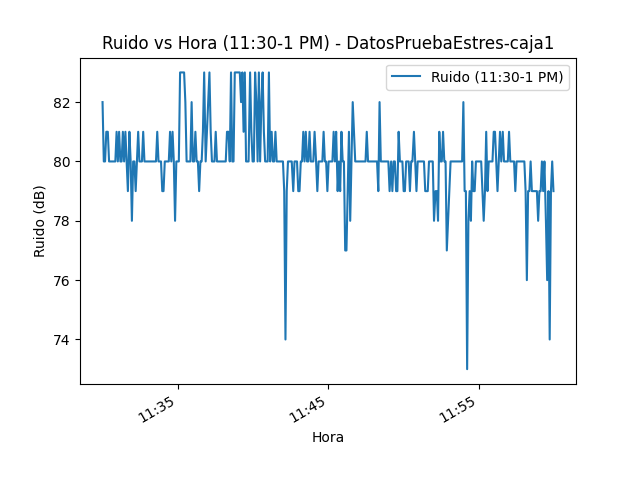
\includegraphics[width=0.8\textwidth]{img/DatosPruebaEstres-caja1_ruido_11-30_1_pm.png}
    \caption{Tercer Periodo de clases}
\end{figure}

\begin{tcolorbox}
    Con un análisis mas profundo y en conocimiento de los periodos de clases, se pueden afirmar los siguientes puntos:
    \begin{itemize}
        \item Durante el primer periodo de clases, el nivel de ruido se mantiene entre 80 y 81 dB, con leves aumentos y grandes disminuciones. Esto podría ser consecuencia de una clase participativa, con momentos de interacción y otros de silencio.
        \item En el segundo periodo de clases, se registran niveles iniciales altos, superando los del primer periodo. Sin embargo, en un punto específico, se observa una disminución continua que finalmente se estabiliza en 80 dB, lo que sugiere que en ese momento se realizó una actividad que requería una reducción moderada del ruido.
        \item En el tercer periodo los niveles de ruido oscilaron entre 80 y 81 dB, lo que podría indicar que la actividad en este periodo fue similar a la del primero, pero con mayores intervalos de silencio o concentración.
    \end{itemize}    
\end{tcolorbox}


\newpage
\textbf{Temperatura}
\begin{figure}[H]
    \centering
    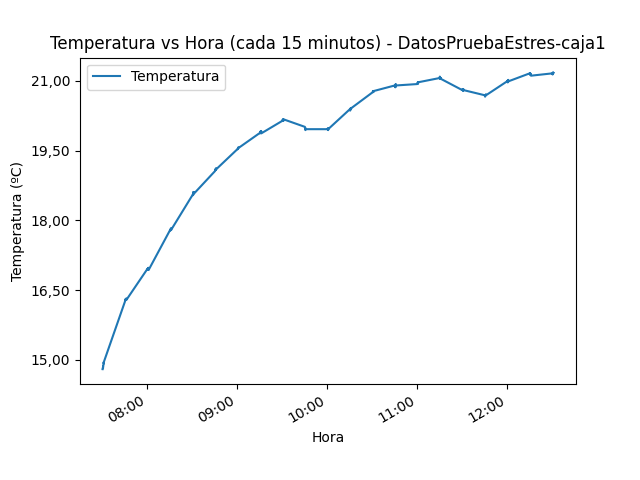
\includegraphics[width=0.8\textwidth]{img/DatosPruebaEstres-caja1_temperatura_vs_hora_15min.png}
\end{figure}

\begin{tcolorbox}
    La gráfica de temperatura del dispositivo 1 muestra un comportamiento esperado: temperaturas bajas por la mañana que aumentan progresivamente a lo largo del día. Al compararla con la gráfica de ruido, podemos inferir que el nivel de ruido podría estar ligeramente influenciado por la temperatura de la sala, aunque el impacto no parece ser significativo.
\end{tcolorbox}

\newpage
\textbf{Humedad}
\begin{figure}[H]
    \centering
    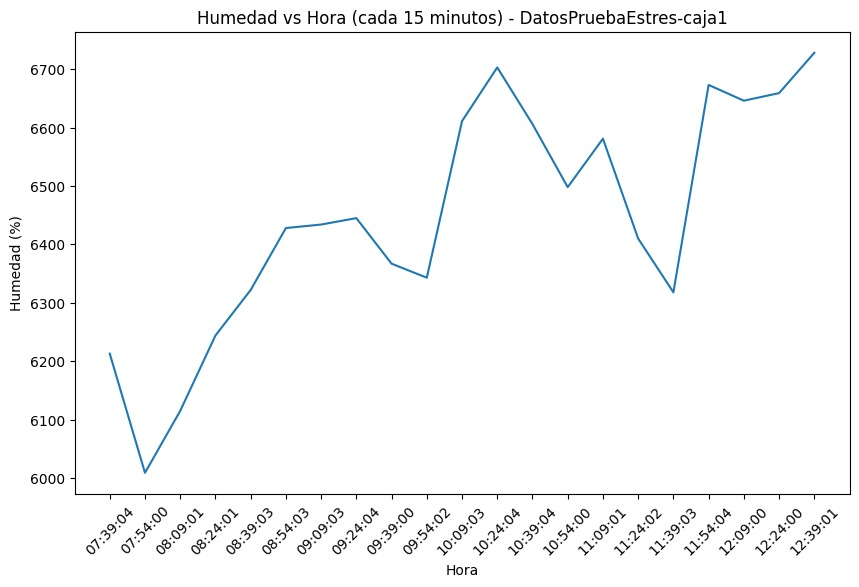
\includegraphics[width=0.8\textwidth]{img/DatosPruebaEstres-caja1_humedad_vs_hora_15min.jpg}
\end{figure}

\begin{tcolorbox}
    En el caso de la gráfica de humedad del dispositivo 1, se observa un inicio con valores altos, posiblemente debido a una interferencia durante la instalación. Posteriormente, los valores se estabilizan en torno a 60, aumentando de manera constante con el tiempo. Además de este incremento general, se detectan disminuciones puntuales que coinciden con los periodos de recreo, lo que sugiere que durante esos momentos se ventiló el aula. Sin embargo, la humedad vuelve a aumentar cuando los ocupantes regresan, y esta tendencia continúa a lo largo del día.
\end{tcolorbox}

\newpage
\textbf{CO2}
\begin{figure}[H]
    \centering
    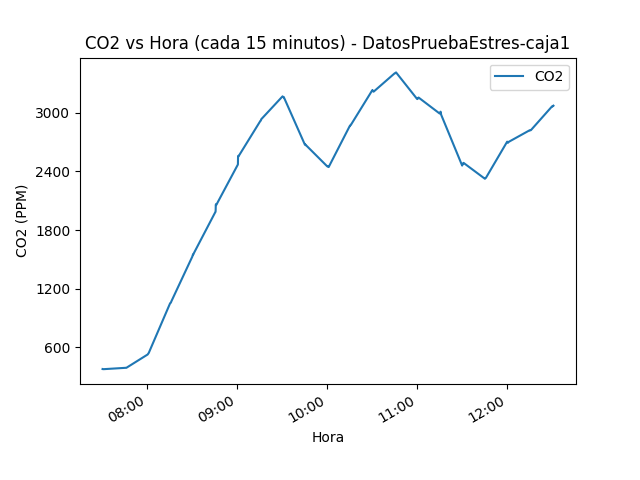
\includegraphics[width=0.8\textwidth]{img/DatosPruebaEstres-caja1_co2_vs_hora_15min.png}
\end{figure}

\begin{tcolorbox}
    La gráfica de concentración de CO2 del dispositivo 1 muestra un comportamiento similar al de la temperatura: valores bajos por la mañana que aumentan progresivamente a lo largo del día. Este aumento puede deberse a la acumulación de CO2 en un espacio cerrado y mal ventilado. Si observamos mas a detalle la gráfica nos damos cuenta que, al igual que con la humedad, esta presenta disminución en los periodos de descaso, indicando una ventilación de la sala a traves de la apertura de puertas o solo algunas ventanas.
\end{tcolorbox}

\newpage
\subsection{Dispositivo 2}

\textbf{Ruido}
\begin{figure}[H]
    \centering
    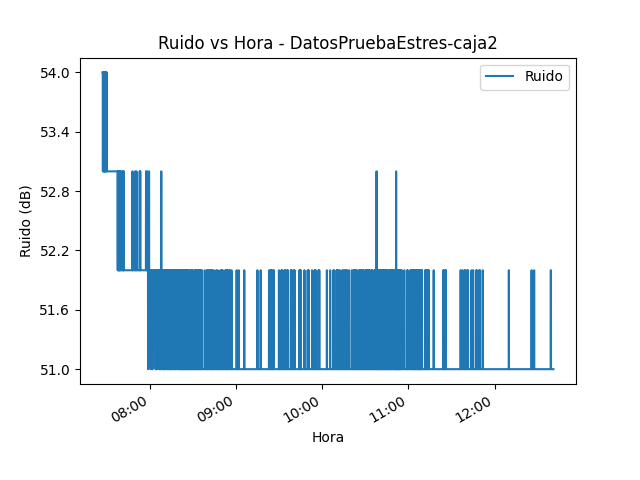
\includegraphics[width=0.8\textwidth]{img/DatosPruebaEstres-caja2_ruido_vs_hora.png}
\end{figure}

\begin{tcolorbox}
    Para el dispositivo 2 y su entorno, podría ser correcto decir que permaneció en un rango de ruido de 50 a 60 dB, lo que indica un nivel de ruido moderado.
\end{tcolorbox}

\newpage
\underline{Graficas por periodos de clases:}

\begin{figure}[H]
    \centering
    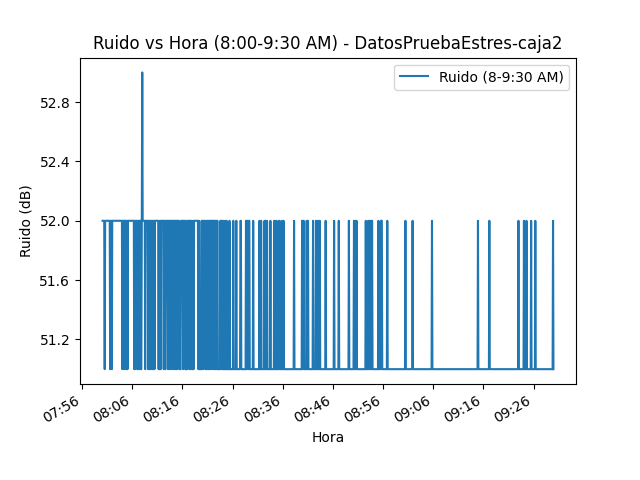
\includegraphics[width=0.8\textwidth]{img/DatosPruebaEstres-caja2_ruido_8_9-30_am.png}
    \caption{Primer Periodo de clases}
\end{figure}

\begin{figure}[H]
    \centering
    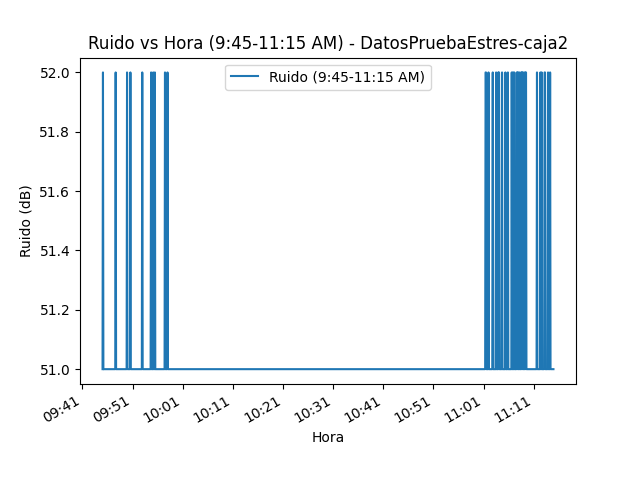
\includegraphics[width=0.8\textwidth]{img/DatosPruebaEstres-caja2_ruido_9-45_11-15_am.png}
    \caption{Segundo Periodo de clases}
\end{figure}

\begin{figure}[H]
    \centering
    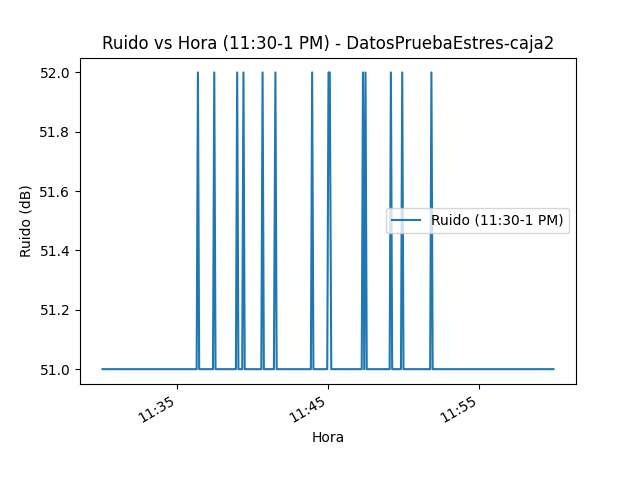
\includegraphics[width=0.8\textwidth]{img/DatosPruebaEstres-caja2_ruido_11-30_1_pm.png}
    \caption{Tercer Periodo de clases}
\end{figure}

\begin{tcolorbox}
    Al realizar un análisis mas detallado del dispositivo 2 y los periodos en los que se registraron los datos, se pueden afirmar los siguientes puntos:
    \begin{itemize}
        \item Los valores se mantienen en los rangos de entre 50 y 53 dB. Estos niveles de ruido presentaron multiples variaciones de entre 50 y 52 dB, con solo un pico de 53 dB.
        \item El segundo periodo presento en su mayoría un nivel constante de 51 dB, con algunas alzas de 1 dB, por lo cual parece correcto afirmar que durante este periodo la aula se vació o se realizo una actividad que requirió silencio.
        \item Al igual que en segundo periodo, el tercer periodo presento un nivel constante de 51 dB, lo que podría indicar que la actividad realizada en este periodo fue similar a la del segundo periodo.
    \end{itemize}
\end{tcolorbox}

\newpage
\textbf{Temperatura}
\begin{figure}[H]
    \centering
    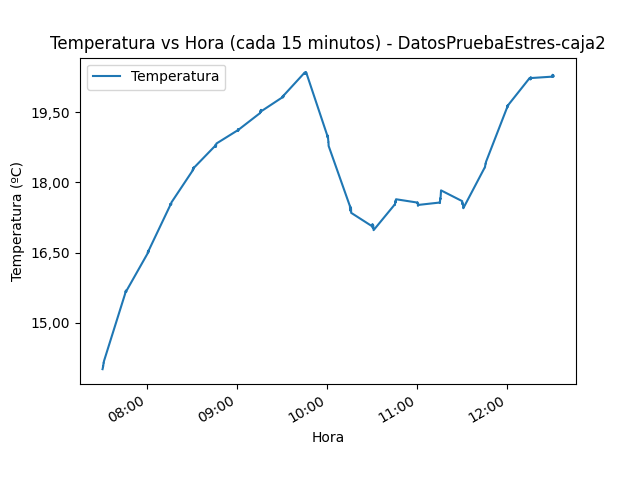
\includegraphics[width=0.8\textwidth]{img/DatosPruebaEstres-caja2_temperatura_vs_hora_15min.png}
\end{figure}
\begin{tcolorbox}
    La gráfica de temperatura del dispositivo 2 muestra un comportamiento similar al del dispositivo 1: temperaturas bajas por la mañana que aumentan progresivamente a lo largo del día. Este ambiente presento la particularidad de que en cierto periodo de tiempo la temperatura disminuyo, lo que podría indicar que durante ese periodo se ventilo la estancia, se abandono el aula, o se activo algún sistema de control de temperatura como un aire acondicionado, ya que al momento que finaliza el periodo de disminución de temperatura, esta se vuelve constante por un periodo de tiempo para luego volver a aumentar.
\end{tcolorbox}

\newpage
\textbf{Humedad}
\begin{figure}[H]
    \centering
    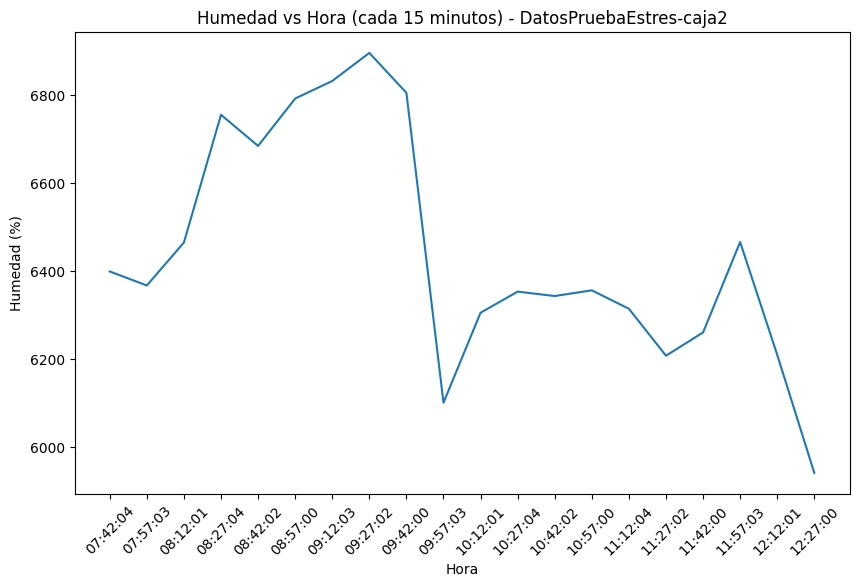
\includegraphics[width=0.8\textwidth]{img/DatosPruebaEstres-caja2_humedad_vs_hora_15min.jpg}
\end{figure}

\begin{tcolorbox}
    La humedad que se observo a traves del dispositivo 2 presenta inicialmente una tendencia a la baja, ya que inicia en un valor alto y luego disminuye. Sin embargo, a partir de cierto periodo la humedad vuelve a aumentar y se mantiene constante en un rango de 66 a 68\%. Este comportamiento puede ser indicativo de la ventilación de la sala, ya que la humedad disminuye cuando se ventila y aumenta cuando se cierra la sala. Al igual que en el dispositivo anterior estos valores se presentan de manera oscilante y con periodos de disminución especifica correspondientes a los periodos de descanso.
\end{tcolorbox}

\newpage
\textbf{CO2}
\begin{figure}[H]
    \centering
    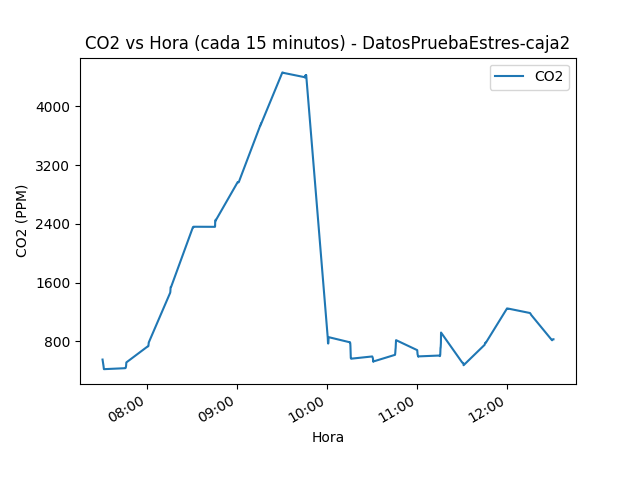
\includegraphics[width=0.8\textwidth]{img/DatosPruebaEstres-caja2_co2_vs_hora_15min.png}
\end{figure}

\begin{tcolorbox}
    Esta gráfica muestra un comportamiento particular, ya que la concentración de CO2 aumenta constantemente hasta un punto en el cual se mantiene constante para luego disminuir. Este comportamiento puede deberse a multiples factores, como a la ventilación del espacio antes mencionado o una disminución en la cantidad de personas presentes en el espacio. Para este espacio se observan peeks de concentración de mas de 4000 PPM, este valor aunque no es peligroso, si es un indicativo de que la ventilación del espacio no fue la adecuada hasta que se tomaron medidas para corregirlo.
\end{tcolorbox}

\newpage
\subsection{Dispositivo 3}

\textbf{Ruido}
\begin{figure}[H]
    \centering
    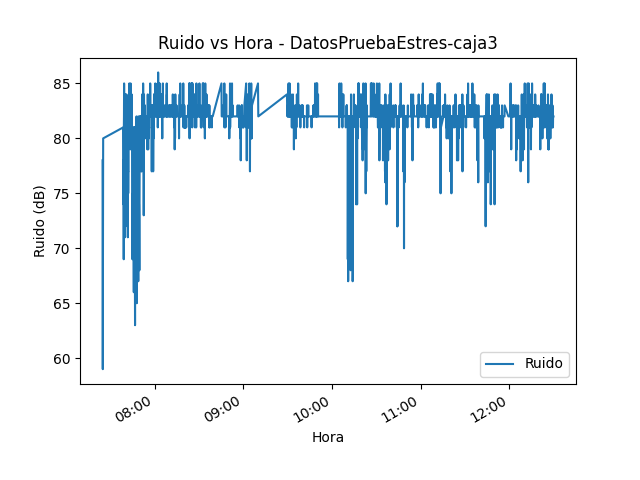
\includegraphics[width=0.8\textwidth]{img/DatosPruebaEstres-caja3_ruido_vs_hora.png}
\end{figure}

\begin{tcolorbox}
    Para el dispositivo 3, a nivel general, observamos niveles de ruido constantes y elevados en niveles de entre 80 y 85 dB.
\end{tcolorbox}

\newpage    
\underline{Graficas por periodos de clases:}
\begin{figure}[H]
    \centering
    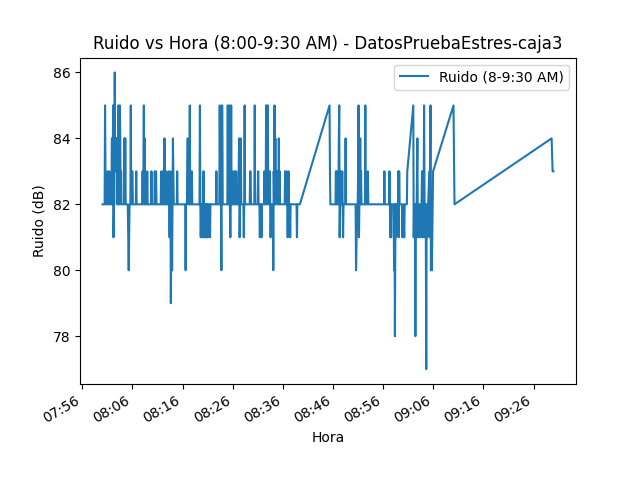
\includegraphics[width=0.8\textwidth]{img/DatosPruebaEstres-caja3_ruido_8_9-30_am.png}
    \caption{Primer Periodo de clases}
\end{figure}

\begin{figure}[H]
    \centering
    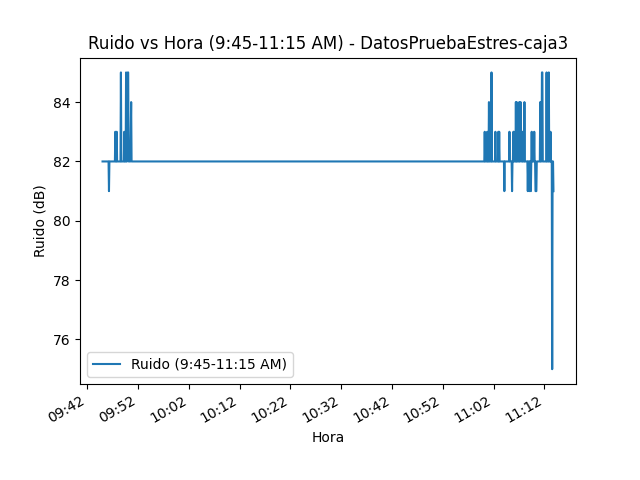
\includegraphics[width=0.8\textwidth]{img/DatosPruebaEstres-caja3_ruido_9-45_11-15_am.png}
    \caption{Segundo Periodo de clases}
\end{figure}

\begin{figure}[H]
    \centering
    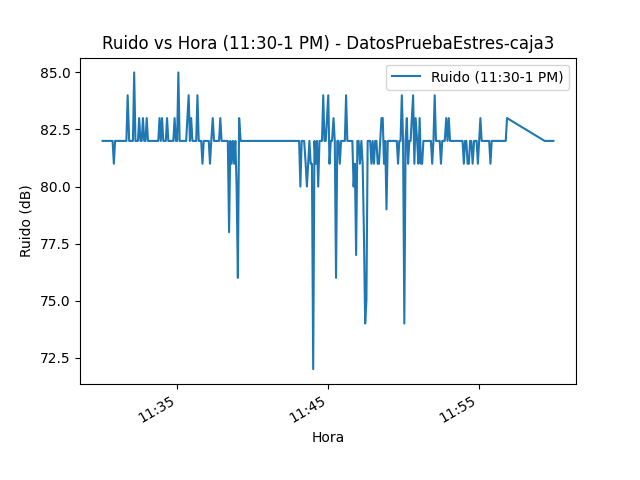
\includegraphics[width=0.725\textwidth]{img/DatosPruebaEstres-caja3_ruido_11-30_1_pm.png}
    \caption{Tercer Periodo de clases}
\end{figure}

\begin{tcolorbox}
    Un análisis mas especifico tomando en cuenta los periodos de clases y niveles de ruido nos otorga los siguientes datos:
    \begin{itemize}
        \item Durante el primer periodo de clases (08:00AM-09:30AM), el ruido se mantiene oscilando entre los 82 y 85 dB, habiendo variaciones de vez en cuando, teniendo como registro máximo 86dB en este periodo y 76dB como el más bajo. Cabe mencionar que hay periodos donde los niveles de ruido tienen un aumento constante, siendo a mitad del periodo y cerca del final del mismo. Se puede inferir que el de mitad del periodo se deba a alguna actividad participativa realizada en clase, mientras que el periodo de aumento cercano al final puede deberse a la misma razón, así como también a que los alumnos se preparan para salir del aula, generando más ruido de lo normal.

        \item El segundo periodo de clases (09:45AM-11:15AM), tiene un ruido constante de 82 dB la mayor parte del tiempo, su registro máximo fue de 85 dB y el menor de 75 dB. Hubo un periodo de silencio entre las 09:52 y las 11:02AM, esto sugiere la realización de alguna actividad realizada en el salón que tiene un ruido moderado, como puede ser una lectura, una explicación extendida por parte del profesor, o el abandono del salón durante ese periodo de tiempo, lo cual explicaría la constante y las variaciones registradas en ese momento.
        
        \item El tercer periodo de clases (11:30AM-01:00PM), el ruido de este suele oscilar en, aproximadamente, los 81 y los 83 dB, siendo su máximo registro de 85 dB y el menor de 72,5 dB. Los registros oscilantes en este periodo sugieren que la actividad dentro de la sala de clases fue variada, teniendo un periodo de participación que dio pie al aumento en los registros y otros de silencio, teniendo una clase variada en los niveles de participación dentro de la sala de clases.
    \end{itemize}
\end{tcolorbox}

\newpage
\textbf{Temperatura}
\begin{figure}[H]
    \centering
    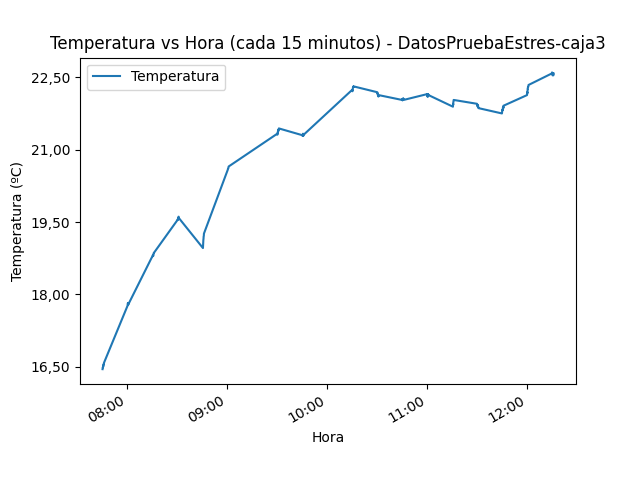
\includegraphics[width=0.8\textwidth]{img/DatosPruebaEstres-caja3_temperatura_vs_hora_15min.png}
\end{figure}

\begin{tcolorbox}
    La gráfica de temperatura del dispositivo 3 muestra un comportamiento similar al de los dispositivos anteriores: temperaturas bajas por la mañana que aumentan progresivamente a lo largo del día. En este caso, la temperatura al llegar a su punto mas alto no presento disminuciones tan visibles como en los dispositivos anteriores; en los periodos de recreo puede apreciarse una leve disminución en la temperatura, siendo la más notoria después del segundo recreo, es decir: durante el periodo del tercer bloque de clases. A través de esto se puede inferir que la ventilación del espacio no fue la adecuada durante el primer recreo y que se realizó durante el tercer periodo mientras se impartían las clases, regulando así un poco el constante aumento en la temperatura. Posiblemente esto se reguló con la apertura de ventanas y puertas dentro de la sala, mejorando así la ventilación en la misma.
\end{tcolorbox}

\newpage
\textbf{Humedad}
\begin{figure}[H]
    \centering
    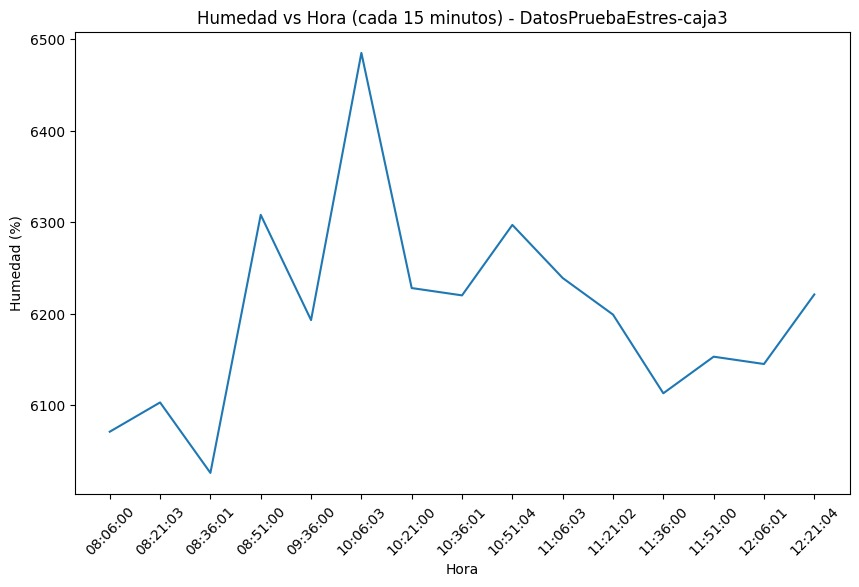
\includegraphics[width=0.8\textwidth]{img/DatosPruebaEstres-caja3_humedad_vs_hora_15min.jpg}
\end{figure}

\begin{tcolorbox}
    La humedad en el ambiente inicia baja, debido a que hay poca afluencia de personas en la sala. A medida que el día avanza, el porcentaje de humedad va en aumento, pero cae rápidamente alrededor de las 10:21AM, apenas elevándose en momentos posteriores. Esto nos indica que hubo una gran cantidad de personas en un tiempo determinado, y contrastando con los datos de CO2 y Temperatura, se puede inferir que aproximadamente en este periodo hubo la mayor afluencia, por lo que la falta de una mayor humedad en este periodo se atribuye a que hubieron individuos en las cercanías del dispositivo, alterando así los resultados del mismo debido a la proximidad.
\end{tcolorbox}

\newpage
\textbf{CO2}
\begin{figure}[H]
    \centering
    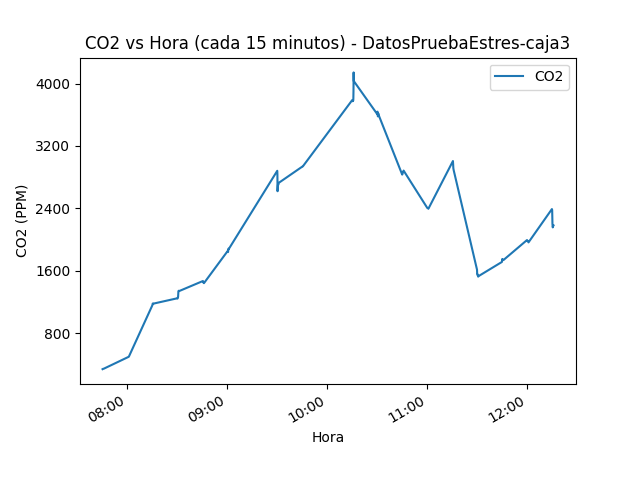
\includegraphics[width=0.8\textwidth]{img/DatosPruebaEstres-caja3_co2_vs_hora_15min.png}
\end{figure}

\begin{tcolorbox}
    Para este dispositivo observamos una tendencia de montaña, ya que aumenta constantemente hasta llegar a la cima, para luego descender. Este comportamiento es el natural esperado en un entorno cerrado y en el cual, al momento de vaciarse o disminuir de afluencia de personas, la concentración de CO2 disminuye. En esta aula se puede afirmar que la ventilación durante el primer periodo de descanso no se llevo a cabo de manera adecuada ya que la concentración de CO2 aumento en lugar de disminuir.
\end{tcolorbox}

\newpage
\subsection{Dispositivo 4}
\textbf{Ruido}
\begin{figure}[H]
    \centering
    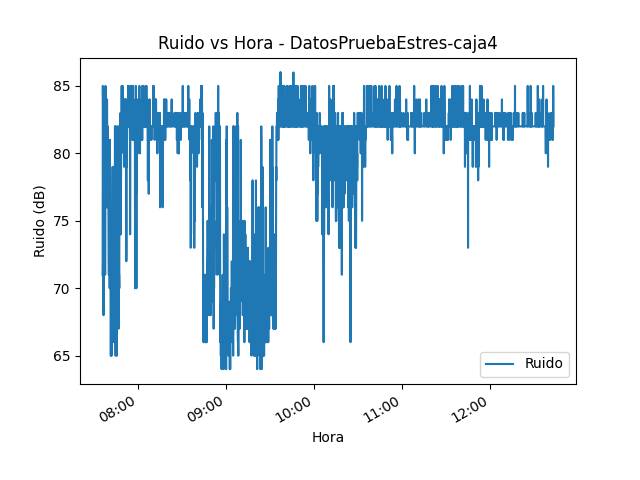
\includegraphics[width=0.8\textwidth]{img/DatosPruebaEstres-caja4_ruido_vs_hora.png}
\end{figure}

\begin{tcolorbox}
    Esta gráfica presenta niveles de ruido en su mayoría altos, sin embargo existen periodos de disminución posiblemente incitados directamente por el ambiente en el cual se encontraba el dispositivo.  
\end{tcolorbox}

\newpage
\underline{Graficas por periodos de clases:}

\begin{figure}[H]
    \centering
    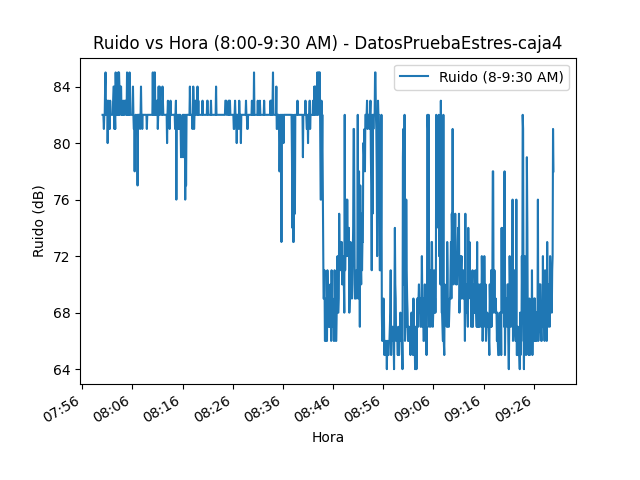
\includegraphics[width=0.8\textwidth]{img/DatosPruebaEstres-caja4_ruido_8_9-30_am.png}
    \caption{Primer Periodo de clases}
\end{figure}

\begin{figure}[H]
    \centering
    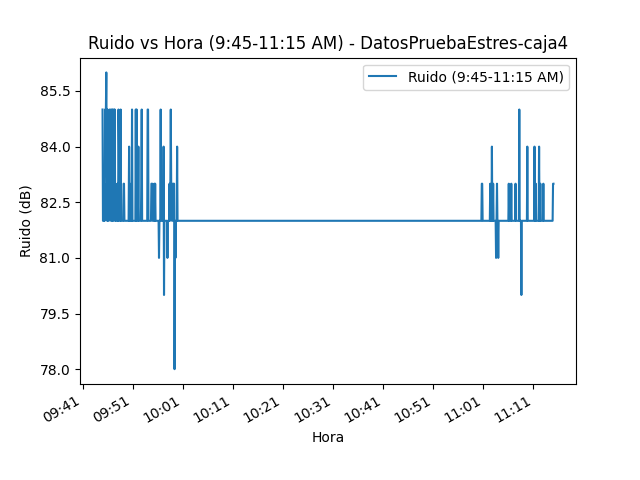
\includegraphics[width=0.8\textwidth]{img/DatosPruebaEstres-caja4_ruido_9-45_11-15_am.png}
    \caption{Segundo Periodo de clases}
\end{figure}

\begin{figure}[H]
    \centering
    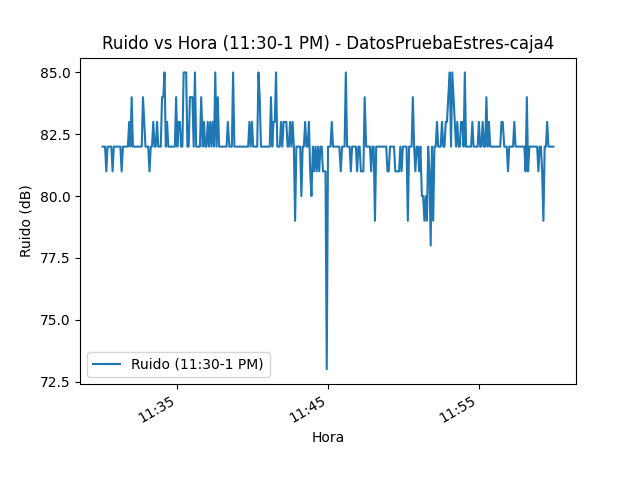
\includegraphics[width=0.8\textwidth]{img/DatosPruebaEstres-caja4_ruido_11-30_1_pm.png}
    \caption{Tercer Periodo de clases}
\end{figure}

\begin{tcolorbox}
    Con un análisis más profundo, teniendo en consideración los periodos de clases, se pueden afirmar los siguientes puntos:
    \begin{itemize}
        \item Durante el primer periodo de clases (08:00AM-09:30AM), el ruido es tiene una tendencia durante la primera mitad de este periodo, tendiendo a estar dentro de los 80 y 85dB y puntos donde baja este registro, siendo 73dB el menor registro durante la primera mitad. Sin embargo, durante la segunda mitad de este primer periodo, no hay un patrón apreciable y el ruido varía demasiado, teniendo puntos donde alcanza los 85dB y otros donde está a 64dB. Sin embargo, debido a que predominan los registros donde los niveles de ruido son inferiores a la primera mitad, es posible inferir que se realiza alguna actividad que los mantiene en relativo silencio, siendo interrumpido de forma constante de alguna manera, probablemente una actividad grupal que les hizo moverse activamente alrededor de la sala de clases, lo cual explicaría los niveles de ruido tan variantes.
        \item El segundo periodo de clases (09:45AM-11:15AM), el ruido registrado en este punto es, en su mayor parte, constantes 82dB, esto debido al periodo de ruido constante entre las 10:01AM y las 11:01AM. Antes y después de ese periodo de silencio, hubo variaciones en los registros, obteniendo el máximo registro de 86dB y el menor de 78dB. Este periodo de ruido constante sugiere una actividad de relativo silencio, como una lectura o explicación extendida por parte del profesor.
        \item Durante el tercer periodo de clases (11:30AM-01:00PM), el ruido de registrado en este suele oscilar entre los 81 y 84dB, su máximo registro es de 85dB y el mínimo de 73dB. Esta variación sugiere una actividad continua dentro de la sala de clases, teniendo periodos cortos de silencio entre medio, por lo que se puede inferir que es un periodo de participación activa dentro de la sala de clases, explicando así los diferentes niveles de ruido en los registros analizados en este periodo.
    \end{itemize}
\end{tcolorbox}

\newpage
\textbf{Temperatura}
\begin{figure}[H]
    \centering
    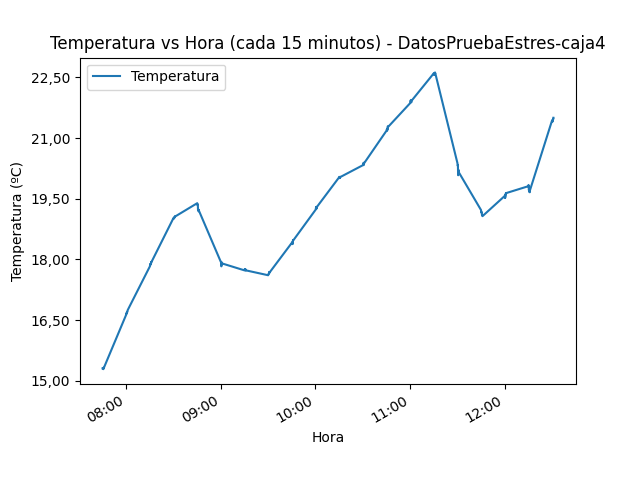
\includegraphics[width=0.8\textwidth]{img/DatosPruebaEstres-caja4_temperatura_vs_hora_15min.png}
\end{figure}

\begin{tcolorbox}
    Al igual que en los casos anteriores observamos temperaturas en aumento. Sin embargo, este presenta un aumento drástico en la temperatura en aproximadamente las 9:45, periodo donde se inicia el segundo bloque de clases, y se mantiene en aumento hasta el término del segundo periodo, luego de eso disminuye durante el segundo recreo y sigue un aumento menor en el periodo de la tercera clase. El aumento drástico de la temperatura es un indicativo de una actividad estimulante, se puede inferir que estos alumnos participaron en alguna clase de educación física durante el primer periodo, resultando en un aumento en la temperatura una vez estos regresaron en el segundo periodo, eso también explicaría el leve aumento durante el primer periodo de clases: casi no habían alumnos en el salón. La ventilación en este caso parece ser adecuada, ya que para el inicio del tercer periodo de clases, la temperatura disminuyó considerablemente.
\end{tcolorbox}

\newpage
\textbf{Humedad}
\begin{figure}[H]
    \centering
    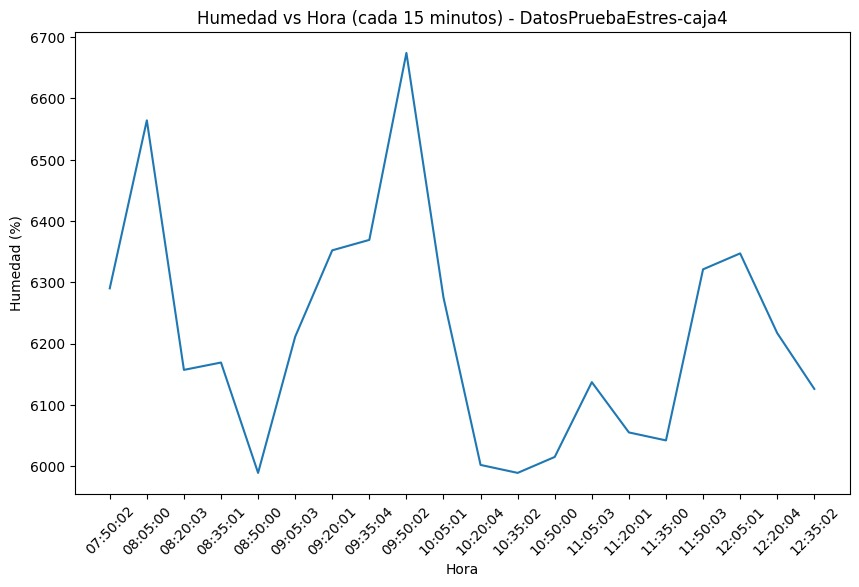
\includegraphics[width=0.8\textwidth]{img/DatosPruebaEstres-caja4_humedad_vs_hora_15min.jpg}
\end{figure}

\begin{tcolorbox}
    Al igual que en los otros casos se observa un comportamiento variado pero con variaciones de 8\% con respecto al inicial y final del periodo de muestreo. Este dispositivo presento la particularidad de que en el primer periodo asignado para descanso, la humedad en lugar de disminuir, aumento de manera considerable, lo que puede indicar que el aula se lleno con mas personas o que la curiosidad de los ocupantes hizo que se acercaran al sensor afectando la lectura verídica de los datos. Esto se sostiene en que al momento de finalizar el periodo de descanso, la humedad disminuyo de manera considerable y vuelve a presentar valores regulares seguidos de una disminución en el segundo periodo de descanso.
\end{tcolorbox}

\newpage
\textbf{CO2}
\begin{figure}[H]
    \centering
    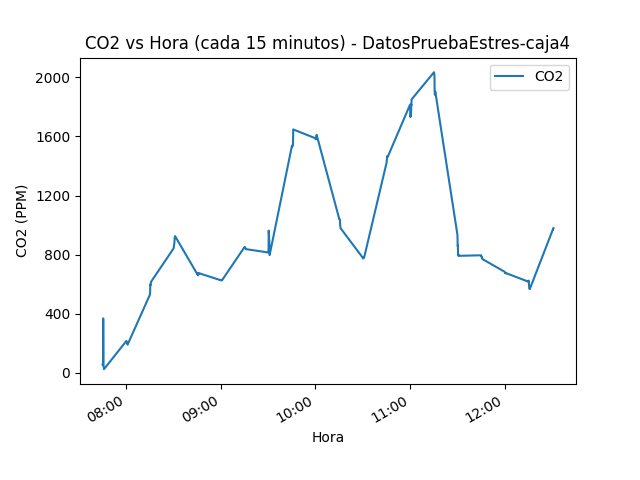
\includegraphics[width=0.8\textwidth]{img/DatosPruebaEstres-caja4_co2_vs_hora_15min.png}
\end{figure}

\begin{tcolorbox}
    Este gráfico nos muestra un comportamiento mas variado pero conservando la tendencia de disminuir en los periodos de receso y aumentar en los periodos de actividad. En este caso se observa que la concentración de CO2 aumento de manera considerable durante el segundo periodo de descanso y disminuyo en picada, indicando una ventilación mas que adecuada.
\end{tcolorbox}

\newpage
\section{Conclusiones}

Como conclusiones generales de los datos obtenidos y las gráficas presentadas, podemos destacar los siguientes puntos:

\begin{itemize}
    \item Los niveles de ruido en algunas de las aulas son elevados y constantes, pero para otras aulas se mantienen en un rango moderado. En general, los niveles de ruido no parecen verse muy influenciados por los otros valores medidos.
    \item La humedad no presenta variaciones significativas en las aulas, sin embargo se observan valores conformes a lo esperado a un ambiente y periodos determinados como lo son un aula de clases y periodos de descanso y actividad.
    \item La temperatura tiene un comportamiento conforme a la temperatura ambiente, durante esta época del año puede no afectar a los ocupantes del espacio, pero en épocas de invierno o verano, la temperatura puede ser un factor determinante.
    \item La concentración de CO2 en ninguna de las aulas presento niveles de extrema preocupación, sin embargo al igual que con la temperatura, en época de verano esta puede verse aumentada de base por lo cual seria imprescindible contar con un monitoreo o con un sistema de control de temperatura.
\end{itemize}

\noindent En resumen, si el monitoreo se realiza de forma continua y en varias locaciones, se podrán identificar patrones y tendencias para su futuro estudio y comprensión.

\end{document}
